\chapter{Сегментація зображення для прискорення алгоритмів стереобачення}

У третьому розділі наведено спосіб прискорення алгоритмів стереобачення
на прикладі алгоритму дифузії за допомогою сегментації зображення.
Представлено практичні результати
застосування алгоритму дифузії з сегментацією
та без із зазначенням вхідних даних.

\section{Сегментація зображення для прискорення алгоритму дифузії}

Зображення розбивається на прямокутку решітку.
Розмір кожної комірки решітки однаковий.

% TODO: add graph size

Назвемо суперпікселем набір пікселів,
які належать до однієї комірки та мають якісь загальні властивості.

Всі пікселі кожної комірки діляться на дві частини, тобто на два суперпікселя,
за середньою інтенсивністю пікселів, які належать до комірки.
До першого суперпікселя відносяться всі пікселі комірки,
інтенсивність яких не перевищує середньої інтенсивності пікселів у цій комірці,
а до другого суперпікселя~---~всі інші пікселі комірки.

% TODO: add formulas with average intensity

Так як пошук карти глибин виконується для лівого зображення,
то сегментується тільки ліве зображення.

Після запропонованої сегментації будується
$\left(m \cdot n \right)$-дольний граф,
де $m$~---~кількість суперпікселів по вертикалі,
$n$~---~кількість суперпікселів по горизонталі.
Тепер кожна доля відповідає одному суперпікселю.
Кожен суперпіксель $\left(y_s, x_s \right)$,
де $1 \leq y_s \leq m, \, 1 \leq x_s \leq n$,
містить $\left| D_{x_s} \right|$ вершин,
що відповідають можливим зсувам, тобто всі пікселі,
що належать одному сіперпікселю,
будуть мати однаку глибину в результуючій карті глибин.

Теперь кожен суперпіксель (або об'єкт) може мати до восьми сусідів:
по два суперпікселя з правої, нижньої, верхньої та лівої комірок решітки,
а також другий суперпіксель, що належить цій же комірці.

% TODO: 3D image for graph
% TODO: Graph size (number of nosed and edges). Comparison with pixel-based graph size

Штраф за вибір мітки $d \in D_{x_s}$ у суперпікселі $\left(y_s, x_s \right)$
задається як сума штрафів за вибір мітки $d$ в усіх пікселяї,
що належать даному суперпікселю
\begin{equation*}
    f_s \left(x_s, y_s, d \right)
    = \sum \limits_{\left(y, x \right) \in \left(y_s, x_s \right)}
        f \left(L \left(y, x\right), R \left(y, x - d \right) \right).
\end{equation*}
Штрафна функція, що накладається на дуги графу, не змінюється.

Таким чином,
штрафна функція задачі \ref{eq:overview:penalty} набуває наступного вигляду
\begin{equation}
\begin{split}
    E_s \left( \overline{d} \right)
    = \sum \limits_{y_s = 1}^{m}
        \sum \limits_{x = 1}^{n}
            f_s \left(x_s, y_s, d \left( x_s, y_s \right) \right) + \\
    + \sum \limits_{y_s = 1}^{m}
        \sum \limits_{x_s = 1}^{n}
            \sum \limits_{\left( y_s', x_s' \right) \in \mathcal{N} \left( y_s, x_s \right)}
            g \left(
                d \left( y_s, x_s \right), d \left( y_s', x_s' \right)
            \right).
\end{split}
\end{equation}

Далі задача розв'язується методом, що описаний у попередньому розділі.

\section{Практичні результати}

Результати роботи програми зображені на рисунку \ref{fig:stereo:pixel}.
Зліва зображена карта глибин, отримана за допомогою алгоритму,
описаного в попередньому розділі, де кожній долі графа відповідає один піксель.
Справа зображена карта глибин,
отримана за допомогою об'єднання частин зображення в суперпікселі.

\begin{figure}[h]
  \centering
  \begin{subfigure}[b]{0.3\textwidth}
      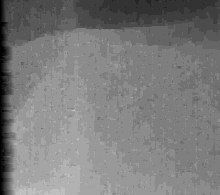
\includegraphics[width=\textwidth]{images/pixel_based_stereo}
      \caption{Карта глибин, отримана алгоритмом дифузії без застосування сегментації зображення}
  \end{subfigure}
  \begin{subfigure}[b]{0.3\textwidth}
      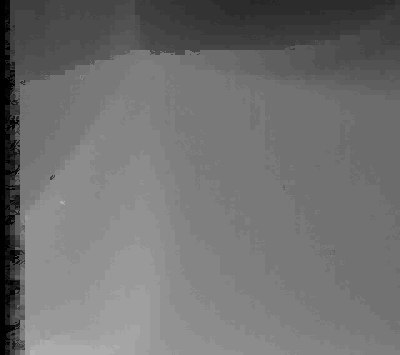
\includegraphics[width=\textwidth]{images/superpixel_based_stereo}
      \caption{Карта глибин, отримана алгоритмом дифузії після застосування сегментації зображення}
  \end{subfigure}
  \caption{Практичні результати}
  \label{fig:stereo:pixel}
\end{figure}

% TODO: launch pixel-based stereo with bigger smoothing term

Вхідні зображення (рис. \ref{fig:stereopair}) були взяті з набору зображень стереопар,
що були зроблені в Міддлберійскому коледжі в 2006 році
\cite{middlebury:ds:1} \cite{middlebury:ds:2}.

\begin{figure}[h]
  \centering
  \begin{subfigure}[b]{0.3\textwidth}
      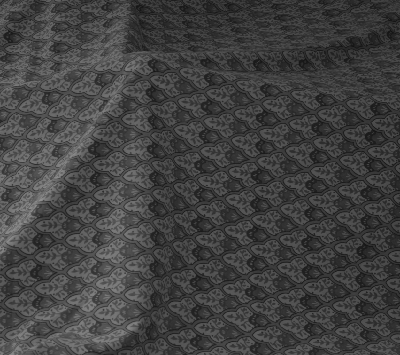
\includegraphics[width=\textwidth]{images/cloth_left_400}
      \caption{Ліве зображення стереопари}
  \end{subfigure}
  \begin{subfigure}[b]{0.3\textwidth}
      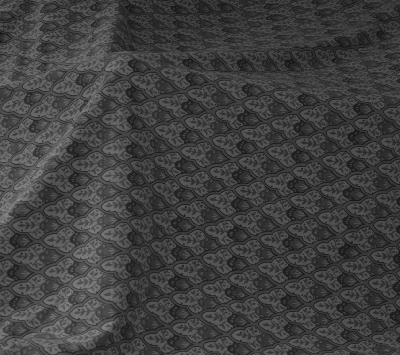
\includegraphics[width=\textwidth]{images/cloth_right_400}
      \caption{Праве зображення стереопари}
  \end{subfigure}
  \caption{Вхідні зображення}
  \label{fig:stereopair}
\end{figure}

Програмне забезпечення
було написано на мові програмування Rust спеціально для цієї роботи.

% Такого результату вдалося досягти за $524$ мілісекунди на компьютері з
% процесором Intel Core i5-3317U, виконавши $28$ ітерацій алгоритму.
% Програмне забезпечення будо написано на Pyhton $2.7$ спеціально для цієї роботи.

\section*{Висновки до розділу 3}
\addcontentsline{toc}{section}{Висновки до розділу 3}

Проведено опис способу прискорення розв'язання задачі стереобачення
за допомогою алгоритма дифузії.
Прискорення алгоритму базується на зменшенні розміру графу,
на якому розв'язується задача, так,
щоб не втратити багато інформації та не погіршити результуючу карту глибин.

% Проведено теоретичний опис ітеративного алгоритму найближчих точок для
% розв'язання задачі, поставленої в першому розділі.
% Алгоритм базується на обчисленні сингулярного розкладу певної матриці,
% тому що цей підхід дає змогу отримати матрицю повороту.
% Виявилося, що в даному випадку сингулярний розклад єдиний з точністю по
% перестановки знаків.
% Отже, невідомі параметри оцінюються однозначно.
% Знайдено розподіл оцінки матриці повороту та доведено,
% що алгоритм завжди зупиняється за скінченну кількість ітерацій.
%
% Для деяких вхідних даних алгоритм дає дуже добрі результати, однак,
% був знайдений простий приклад, для якого алгоритм не працює задовільно.
% Таким чином, необхідні подальші дослідження,
% щоб виявити ще слабкі та сильні сторони алгоритму.
